%% This is an example first chapter.  You should put chapter/appendix that you
%% write into a separate file, and add a line \include{yourfilename} to
%% main.tex, where `yourfilename.tex' is the name of the chapter/appendix file.
%% You can process specific files by typing their names in at the 
%% \files=
%% prompt when you run the file main.tex through LaTeX.
\chapter{WebAuthn Firewall Design}\label{Chap:WebauthnFirewallDesign}

This chapter describes the high-level design and purpose of \sys{}, the WebAuthn firewall, and how it fits within an existing web application. It also describes how a software engineer would use the different configuration options and tools that \sys{} provides in order to secure a web service.

\section{Overview}

\sys{} acts as a Web Application Firewall. It is situated directly between the frontend and backend, processing all user requests sent between the two. At the highest-level, the purpose of \sys{} is to map HTTP requests on protected routes to authentication messages and then verify those requests. To make the mapping and verification easier, \sys{} provides configurable options, a domain specific language and a collection of default functions.

\subsection{Request Life Cycle}

\begin{figure}[h]
  \centering
  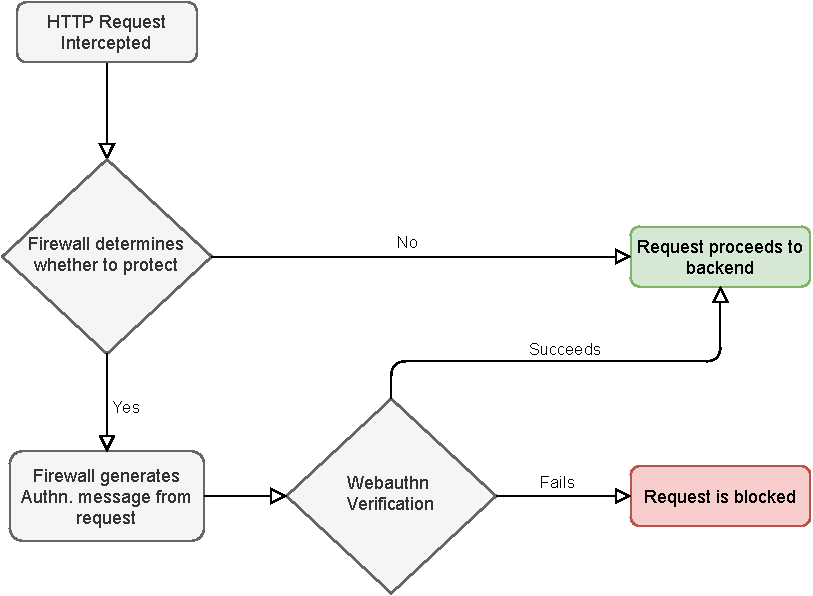
\includegraphics[width=12cm]{HTTP_request_flow_drawio}
  \caption{The decision process for authorizing an HTTP request or not.}  
  \label{fig:RequestLifeCycle}
\end{figure}

The flowchart in Figure~\ref{fig:RequestLifeCycle} illustrates the life cycle of an HTTP request passing through the WebAuthn firewall. It begins with \sys{} capturing and parsing it when it is sent from the frontend to the backend. Then \sys{} decides whether to verify those requests with transaction authentication or not. If not, the request is simply proxied through to the backend without any extra work. Otherwise, it performs a verification procedure on the request and only upon success does the request pass through the firewall to the backend. Upon failure, the request is blocked.

\subsection{Securing Sample Operation}

To illustrate how an operation is secured, consider the example of an HTTP request to delete an SSH key within Gogs named \lstinline{"Damian's SSH Key"}. Code Snippet~\ref{code:deleteSSHKeyRequest} is the HTTP request and relevant parts of its payload.

\begin{lstlisting}[float=h,label=code:deleteSSHKeyRequest,caption=A sample HTTP request to delete the SSH key with ID 6.] 
route: "user/settings/ssh/delete",
form-data: {
  id: 6,
  assertion: "<assertion data from hardware authenticator>"
}
\end{lstlisting}

This request should map to a human readable authentication message, in particular: \lstinline{"Delete SSH key named: Damian's SSH Key"}. Notice that the HTTP request contains the ID of the SSH key, but not the name itself. The name is not present anywhere in the request, but can be contextualized by the ID from the backend as described in Section~\ref{Sec:ContextRetrieval}. The domain specific language and default functions make this mapping and context retrieval easier. Code Snippet~\ref{code:deleteSSHKey} is roughly what manually securing this route in Go would look like.

\begin{lstlisting}[float=h,label=code:deleteSSHKey,caption=Route handler which manually secures the delete SSH key operation of Gogs.] 
func deleteSSHKey(w http.ResponseWriter, r *http.Request) {
  id := int(r.Form["id"])
  assertion := r.Form["assertion"]

  // Retrieve the SSH key name of `id`
  var sshKeyInfo struct {
    KeyName string `json:"keyname"`
  }
  PerformRequestJSON(fmt.Sprintf("server_context/ssh_key/%d", id),
                     &sshKeyInfo)

  authText := fmt.Sprintf("Delete SSH key named: %s", 
                          sshKeyInfo.KeyName)

  // Check the `assertion` against the `authText`
  FinishLogin(assertion, authText)
}

router.HandleFunc("/user/settings/ssh/delete", 
                  deleteSSHKey).Methods("POST")
\end{lstlisting}

%% 
%% \iffalse
%%  then performs an HTTP access to the backend's context route to retrieve a JSON object of the SSH key represented by \lstinline{"id"}. 
%% \fi
%% 

First, the code reads the \lstinline{"id"} and \lstinline{"assertion"} values from the request form-data. It then contextualizes the \lstinline{"id"} to retrieve the name of the associated SSH key via the backend's context route. Finally, it creates an authentication message and verifies it against the \lstinline{"assertion"} data. This handler is attached to the HTTP route for SSH key deletion.

The domain specific language and default functions simplify this code. The HTTP route for SSH key deletion, \lstinline{"/user/settings/ssh/delete"}, and request type, \lstinline{"POST"}, are specified in one function call. A short domain specific program specifies how to generate the authentication message. It begins with a format string \lstinline{"Delete SSH key named: %v"} where the format tag \lstinline{"%v"} gets substituted with the SSH key name. Code Snippet~\ref{code:DSLdeleteSSHKey} is the firewall code that secures the SSH key deletion for Gogs.

%% 
%% \iffalse
%% Simpler code makes development and maintenance of the webauthn firewall much easier.

%% blueprints

%% The domain specific program accepts a format string with substitutable format tags to build the authentication message. 
%% \fi
%% 

\begin{lstlisting}[float=h,label=code:DSLdeleteSSHKey,caption=Gogs firewall code which incorporates the domain specific language to secures the delete SSH key operation.]
Secure("POST", "/user/settings/ssh/delete", 
  Authn("Delete SSH key named: %v",
    wf.SetContextVar("ssh_key", wf.Get("id")),
    wf.GetVar("ssh_key").SubField("Name"),
))
\end{lstlisting}

As demonstrated above, the traditional method of directly integrating WebAuthn into a web service is bulky and difficult to configure. \sys{} allows an engineer to write less code to achieve the same functionality, thus making development easier and less error-prone.

%% 
%% \iffalse
%% The chief task is to simplify integrating webauthn transaction authentication into a web service.

%% to develop and get that code correct.

%%The firewall is designed to be highly configurable and minimally intrusive. The less code an engineer has to modify in the web service itself, the better.
%% \fi
%% 

\subsection{Configurable Components}

\begin{figure}[h]
  \centering
  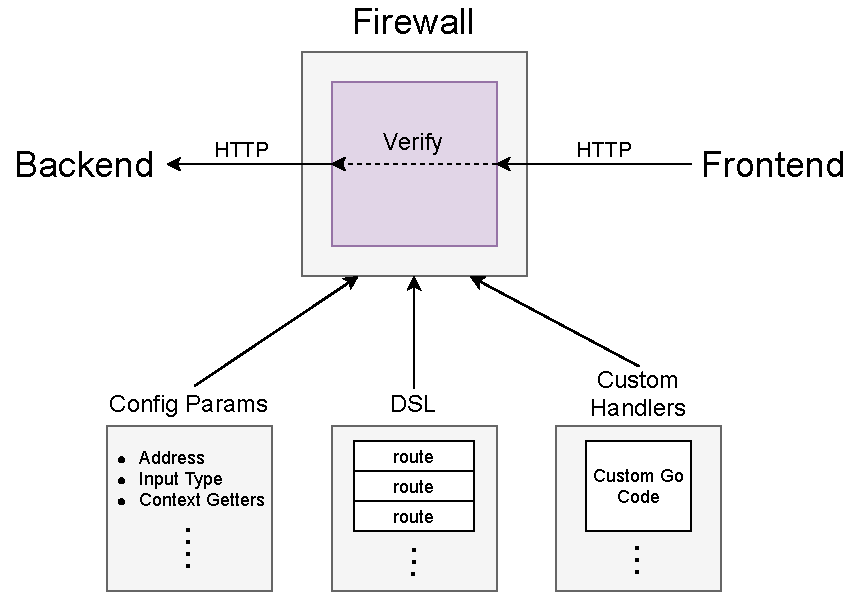
\includegraphics[width=14cm]{firewall_configuration_drawio}
  \caption{The functionality of the WebAuthn firewall fully depends on the configurable components passed into it.}
  \label{Fig:ConfigurableComponents}
\end{figure}

Two sources of configuration enable the \sys{}'s customizable nature. One source is the central configuration element depicted as the leftmost input block in Figure~\ref{Fig:ConfigurableComponents}. It contains the general configurable parameters, from which a number of core WebAuthn routes are deduced and provided automatically.

The other two input blocks of Figure~\ref{Fig:ConfigurableComponents} handle the rest of the application specific routes to be secured. They are secured either using the domain specific language or custom Go code. These configurable options can be easily modified to completely define how \sys{} protects a web service. 

%% 
%% \iffalse
%% Lastly, any route not covered by a domain specific program may be secured using custom handler code utilizing the full power of the Go programming language.

%% come together in the firewall to enable its function. There is a central configuration element for the whole firewall. 

%% A number of core webauthn routes that are provided automatically by the firewall. The rest of the application specific routes are configured using a domain specific language or custom Go code. 

%% The components of the firewall that enable its customizable functionality can be divided into two categories.

%%  by the firewall according to these configurations. 
%% \fi
%% 

Apart from configuration ease, the design of a WebAuthn firewall is powerful because it is almost transparent to the web service it is securing. The backend is unaware that the requests it receives are WebAuthn authenticated. The frontend has to interface with the user's hardware authenticator device, so it must be aware of WebAuthn, but only to a minor extent. As a result, deployment of \sys{} is simple and seamless.

%% 
%% \iffalse
%% it needs transaction authentication, the firewall acts as a gatekeeper for that request.


%% Each request gets parsed by the firewall, and understood whether it is a request that needs webauthn transaction authentication or not. If not, the request is simply proxied through to the backend without any extra work. However, if it needs transaction authentication, the firewall acts as a gatekeeper for that request. The firewall performs a verification procedure on the request and only upon success does the request pass through the firewall to the backend. If it fails, the firewall returns an error back to the frontend. This design strategy for integrating webauthn transaction authentication into a service is very powerful because it is web service agnostic. The backend is completely unaware that the requests it receives are webauthn authenticated. Of course, since the frontend has to interface with the user's hardware authenticator device, it must be aware of webauthn, but only to a minor extent. 
%% \fi
%% 

\section{Proxying Requests}\label{Sec:ProxyingRequests}

In three different case studies, \sys{} is used to integrate WebAuthn transaction authentication into two different paradigms of web service designs, RESTful and server-side rendered websites. For each, the notion of the firewall being situated between the frontend and backend is slightly different, but the function and role of \sys{} is the same, filtering, verifying and proxying requests. 

\begin{figure}[h]
  \centering
  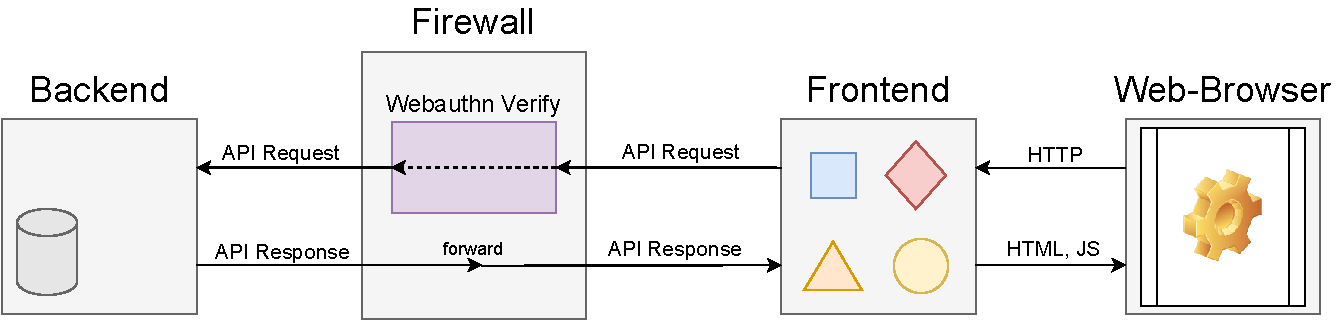
\includegraphics[width=\textwidth]{RESTful_with_firewall_drawio}
  \caption{The positioning and role of the WebAuthn firewall in a RESTful paradigm web service.}
  \label{Fig:ProxyingRequestsRESTful}
\end{figure}

%% 
%% \iffalse
%% and backend are separate programs running on their own IP addresses and ports. The user's web-browser interacts with the frontend through its IP address.
%% \fi
%% 

For a RESTful web application, the placement of the firewall is more intuitive. As depicted in Figure~\ref{Fig:ProxyingRequestsRESTful}, the firewall sits between the frontend and backend of the web service. In a RESTful design, the frontend runs in the web-browser and renders the webpage visible to the user. Whenever the frontend needs to interact with the backend, it launches HTTP requests to the IP address of the backend. However, since \sys{} is situated between the two and runs on its own IP address, the frontend must be reconfigured to use \sys{} as its destination target address. So when the frontend needs to issue a backend request, it sends it to \sys{} rather than to the backend. From there, as represented by the ``Firewall'' box in Figure~\ref{Fig:ProxyingRequestsRESTful}, the firewall performs its role and, as necessary, proxies onward to the actual backend. Responses from the backend are returned to the firewall which are automatically forwarded on to the frontend. 

\begin{figure}[h]
  \centering
  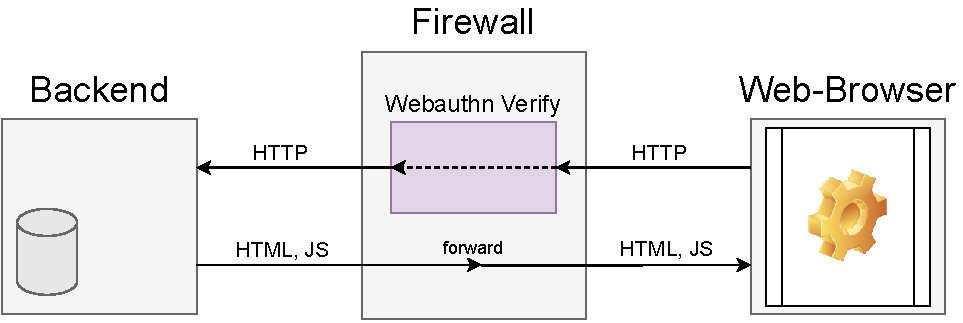
\includegraphics[width=\textwidth]{ServerSide_with_firewall_drawio}
  \caption{The positioning and role of the WebAuthn firewall in a server-side rendering paradigm web service.}
  \label{Fig:ProxyingRequestsServerSide}
\end{figure}

In a server-side rendering web application, there is no notion of a frontend rendering the webpage like in the RESTful use case. Rather, every webpage visible to the user is generated by the backend and sent to the web-browser. From the web-browser, the webpage interacts directly with the IP address of the backend. With the WebAuthn firewall in place as shown in Figure~\ref{Fig:ProxyingRequestsServerSide}, the endpoint of the webpage is configured to be the address of \sys{} instead of the backend. This way, all HTTP requests that originate from the webpage are sent to \sys{}. The firewall processes these requests and relays them onward to the server-side rendering web application if the WebAuthn verification code passes. In such a setup, the WebAuthn firewall is situated between the web-browser's webpage and backend.

%% 
%% \iffalse
%% and are directed to the firewall.

%% the firewall additionally performs the role of the frontend described in the RESTful use case. As shown in Figure~\ref{Fig:ProxyingRequestsServerSide}, the user's web-browser interacts with the IP address of the firewall directly. All HTTP requests originate from the user's web-browser and are directed to the firewall. In a server-side rendering web application, the webpage rendering code and backend use the same address. The firewall processes requests sent to it and relays them onward to the server-side rendering web-application if the verification code passes. In such a setup, the WebAuthn firewall is situated between the web-browser and backend.
%% \fi
%% 

%% 
%% \iffalse
%% However with the webauthn firewall, requests are sent 

%% So requests that are sent to the firewall, which does its role and, if necessary, relays onward to the server-side rendering web-application. In this case, the webauthn firewall is situated between the web-browser and backend. But nonetheless, it is the same principle as with the RESTful web application use case. An origin, in this case the web-browser, issues requests destined for a backend, but the firewall intercepts them, before they continue on if everything succeeds.
%% \fi
%% 

\section{WebAuthn Firewall Configuration}

%% TODO: Make option in firewall to either pass through or block non-specified requests. Modify this paragraph

Some HTTP requests need to be transaction authenticated first before passing through the WebAuthn firewall. The software engineer configures \sys{} to select which requests to verify and what their authentication messages should be. This is done by including the route in \sys{}'s configuration. All other routes not specified in the configuration are simply passed on through to the backend without any checks.

%% 
%% \iffalse
%% the webauthn firewall filters requests sent to it, 

%% Which requests get held back and what their authentication messages are is configured in the firewall by the software engineer. 

%% As HTTP requests pass through the webauthn firewall, some need to be webauthn transaction authenticated first. 

%% In order to specify which HTTP route gets filtered and transaction authenticated, the engineer simply includes the route in the firewall's configuration.
%% \fi
%% 

\subsection{Configuration Parameters}\label{Sec:ConfigurationParameters}

\sys{} has a number of configurable parameters that aid and dictate how routes are secured. Code Snippet~\ref{code:ConduitConfiguration} is the firewall configuration for Conduit.

\begin{lstlisting}[float=h,label=code:ConduitConfiguration,caption=The firewall configuration for the Conduit web service.]
  firewallConfigs := &wf.WebauthnFirewallConfig{
    FrontendAddress:       frontendAddress,
    ReverseProxyTargetMap: reverseProxyTargetMap,
    ReverseProxyAddress:   reverseProxyAddress,

    GetUserID: userIDFromJWT,
    ContextGetters: wf.ContextGettersType{
      "comment":      commentFromCommentID,
      "article":      articleFromArticleSlug,
      "current_user": getCurrentUser,
    },

    WebauthnCorePrefix: "/api/webauthn",
    LoginURL:           "/api/users/login",
    LoginGetUsername: func(r *wf.ExtendedRequest) (string, error) {
      return r.Get_WithErr("user", "username")
    },
  }
\end{lstlisting}

The fields within the configuration are grouped by function. The WebAuthn library uses the first group, \lstinline{RPDisplayName} and \lstinline{RPID}, when setting up and verifying transaction authentication events. 

\begin{figure}[h]
  \centering
  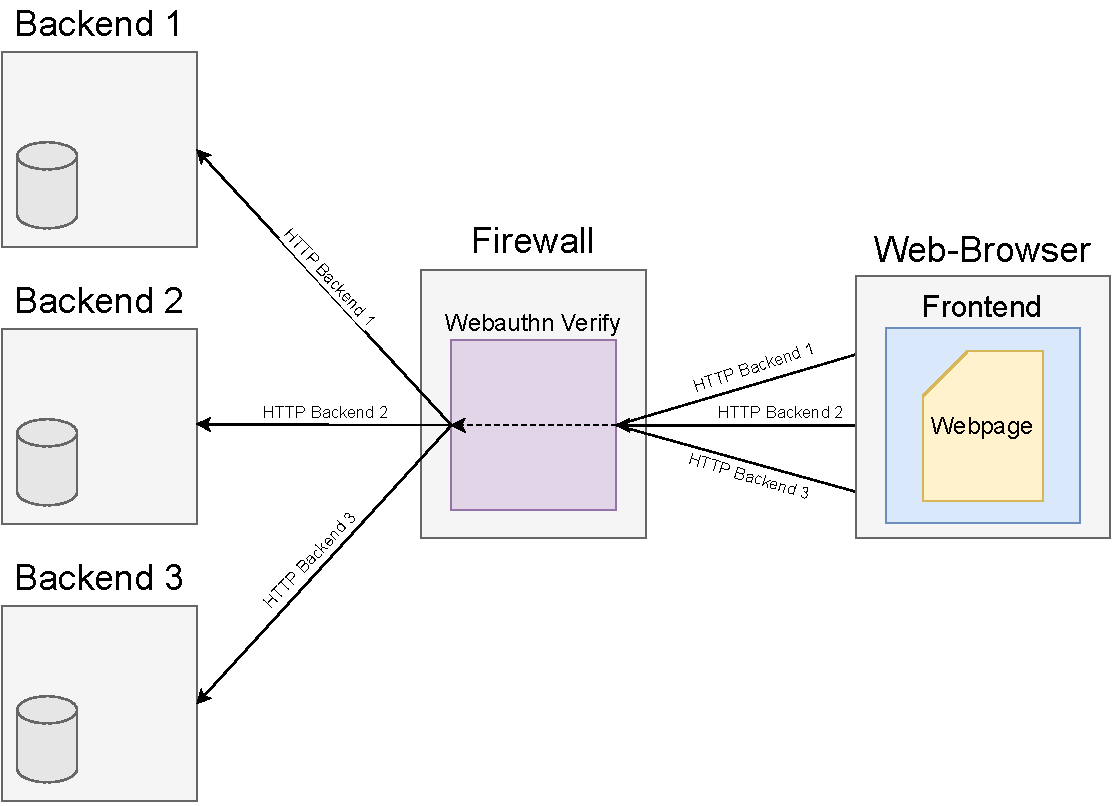
\includegraphics[width=14cm]{multitarget_RESTful_drawio}
  \caption{A WebAuthn firewall handles multiple backend targets for a single frontend.}
  \label{Fig:MultiTargetRESTful}
\end{figure}

The second group, \lstinline{FrontendAddress}, \lstinline{ReverseProxyTargetMap} and \lstinline{ReverseProxyAddress}, contains the proxying address information. They hold the address of the frontend, the target backends and the firewall itself, respectively. It is possible for a web service's frontend to access multiple backends. In this case, the firewall must know which backend to forward incoming requests to after processing them. This is stored as a hash map of hosts and target backends in \lstinline{ReverseProxyTargetMap}. This field simply configures the firewall, as illustrated in Figure~\ref{Fig:MultiTargetRESTful}, to catch requests of a given \lstinline{host} address and forward them to a specific \lstinline{target}.

%% 
%% \iffalse
%% \begin{itemize}[nosep]
%% \item \lstinline{FrontendAddress}: Set to the frontend address. In a RESTful context, that is the frontend itself. In a server-side context, since the firewall functions as the frontend, it should be the firewall's address.

%% \item \lstinline{ReverseProxyTargetMap}: A hash map of hosts and targets, along with their respective default input getters described in Section~\ref{Sec:DefaultInputGetters}. This field configures the firewall to catch requests of a given \lstinline{host} and forward it to a specific \lstinline{target}. There are separate default input getters since requests going to different hosts may have different representations of their payloads. The following code snippet is the \lstinline{ReverseProxyTargetMap} from the firewall configuration for Calypso.

%% \item \lstinline{ReverseProxyAddress}: Set to the address where the firewall should attach and listen on.
%% \end{itemize}

%% \begin{lstlisting}
%% // wf.NewProxyTarget(host, target, defaultInputGetter)
%% reverseProxyTargetMap = 
%%   wf.NewProxyTarget("public-api.wordpress.com", 
%%                     "https://workaround-public-api.wordpress.com", 
%%                     wf.GetJSONInput).
%%   AnotherTarget("wordpress.com", 
%%                 "https://workaround.wordpress.com",
%%                  wf.GetFormInput)
%% \end{lstlisting}

%% In this case, requests destined for \lstinline{"public-api.wordpress.com"} get forwarded to \\ \lstinline{"https://workaround-public-api.wordpress.com"} and have JSON payloads. Requests destined for \lstinline{"wordpress.com"} get forwarded to \lstinline{"https://workaround.wordpress.com"} and have form-data inputs. 
%% \fi
%% 

%% 
%% \iffalse
%% The \lstinline{FrontendAddress} should naturally be set to the

%% The \lstinline{ReverseProxyTargetMap} is a hash map of hosts and targets, along with their respective default input getters described in Section~\ref{Sec:DefaultInputGetters}. This field tells the firewall to catch requests of a given \lstinline{host} and forward it to a specific \lstinline{target}. There are separate default input getters since requests going to different hosts may have different representations of their payloads. The following is the \lstinline{ReverseProxyTargetMap} from the firewall configuration for Calypso:

%% The \lstinline{ReverseProxyAddress} should be set to the address where the firewall should attach itself and listen on.
%% \fi
%% 

The third group is for context retrieval, explained in greater detail in Section~\ref{Sec:ContextRetrieval}. During normal operation of the firewall, such as verifying incoming HTTP requests, it is often useful to identify the current user issuing that request. For example, the public key credential of a user are stored under their ID in \sys{}'s database. 

Since determining the current user's ID is application specific, the \lstinline{GetUserID} is left to the engineer to supply. The example configuration above implements a function that extracts the current user's ID from the JSON Web Token (JWT) included in the HTTP request headers.

Constructing an authentication message oftentimes needs more context than supplied in the HTTP request. The \lstinline{ContextGetters} is a collection of context getter functions written by the engineer. Essentially, they retrieve supplemental information needed to generate the authentication message of a protected HTTP request in a human-readable form. When setting up routes to protect, there is a clean way in the domain specific language to invoke these functions to fetch more context as needed.



%% 
%% \iffalse
%% For example, a request may contain an object ID, but to construct the authentication message, the name of the object is needed. The \lstinline{ContextGetters} is a collection of context getter functions written by the engineer. These context getter functions would translate the object ID to the object itself, usually involving a supplemental HTTP request to the backend. Then when setting up routes to protect, there is a clean way in the domain specific language to invoke these functions to retrieve more context as needed.

%% Section~\ref{Sec:ContextRetrieval} explains the context getter functions in greater detail. 

%% \fi
%% 

%% 
%% \iffalse
%% \begin{itemize}[nosep]
%% \item \lstinline{GetUserID}: A function that, given an HTTP request, extracts the current logged in user's ID. Since this is very application specific, it is up to the engineer to implement this function. The example configuration above implements a function that extracts the current user's ID from the JSON Web Token (JWT) included in the HTTP request headers.

%% \item \lstinline{ContextGetters}: A hash map of context tags and context getter functions. When the engineer sets up routes to protect, there is a clean way to invoke these functions by tag to retrieve more context as needed.
%% \end{itemize}
%% \fi
%% 

%% 
%% \iffalse

%% The \lstinline{GetUserID} is a function that, given an HTTP request, extracts the current logged in user's ID. Since this is very application specific, it is up to the engineer to implement this function. The \lstinline{ContextGetters} is a hash map of context tags and context getter functions. When the engineer sets up routes to protect, there is a clean way to invoke these functions by tag to retrieve more context as needed.

%% \fi
%% 

The fourth group configures the default handlers, explained in more detail in Section~\ref{Sec:DefaultHandlers}. When integrating WebAuthn into a service, there are a number of operations that are a core part of the WebAuthn protocol. They are related to the WebAuthn registration event, the setup event, user login and WebAuthn disable. These fields provide the default handlers with just enough information such that they can be tailored for the given web service.

%% 
%% \iffalse
%% \begin{itemize}[nosep]
%% \item \lstinline{WebauthnCorePrefix}: Specifies the prefix for all URL routes of core webauthn events. In this case, for example, the webauthn setup route is found at \lstinline{"/api/webauthn/begin_attestation"}.

%% \item \lstinline{LoginURL}: The url route where the applications POSTs to during login.

%% \item \lstinline{LoginGetUsername}: A special function that extracts the username from the login HTTP request's payload.

%% \end{itemize}
%% \fi
%% 

%% 
%% \iffalse

%% The \lstinline{WebauthnCorePrefix} specifies the prefix for all URL routes of core webauthn events. In this case, for example, the webauthn setup route is found at \lstinline{"/api/webauthn/begin_attestation"}. The \lstinline{LoginURL} is the url route where the applications POSTs to during login. The \lstinline{LoginGetUsername} is a special function that extracts the username from the login HTTP request's payload.

%% \fi
%% 

The final group contains miscellaneous parameters. Sometimes a web service's frontend expects the HTTP OPTIONS for every URL route it interacts with. The \lstinline{SupplyOptions} flag controls whether \sys{} should supply OPTIONS for every protected route.

%% 
%% \iffalse
%% \begin{itemize}[nosep]

%% \item \lstinline{SupplyOptions}: A boolean flag specifying whether protected routes should respond with an HTTP OPTIONS verb or not.

%% \item \lstinline{Verbose}: A boolean flag specifying whether the firewall should log the HTTP requests it processes.

%% \end{itemize}
%% \fi
%% 

%% 
%% \iffalse

%% The \lstinline{SupplyOptions} is a boolean flag specifying whether protected routes should respond with an HTTP OPTIONS verb or not. The \lstinline{Verbose} is a boolean flag specifying whether the firewall should log the HTTP requests it processes.

%% \fi
%% 

\subsection{Default Input Getters}\label{Sec:DefaultInputGetters}

An HTTP request may contain and encode its payload in a variety of ways. \sys{} supplies four default input getter functions that extract values from requests in different formats. Each default input getter follows the same API, so new ones can be implemented easily as necessary. The getters include:

\begin{itemize}[nosep]
\item \lstinline{GetFormInput}: Parses form-data request payloads.

\item \lstinline{GetJSONInput}: Parses JSON request payloads.

\item \lstinline{GetURLInput}: Parses values stored in the HTTP request url. An example would be \lstinline{"/user/comment/6"} parsing the comment ID \lstinline{6} from the URL.

\item \lstinline{GetURLParamInput}: Parses parameters passed along with the HTTP request url. An example would be \lstinline{"/user/comment?id=9"} parsing the comment ID \lstinline{9} from the URL.

\end{itemize}

\subsection{Context Retrieval}\label{Sec:ContextRetrieval}

%% TODO maybe include some image, incoming ID in request, firewall gets context

When an HTTP request contains non-human friendly identifiers that need to be understood by the user, those identifiers must be translated to their human readable counterparts. For example, an ID identifies a user's comment to a blog post in the Conduit application. Showing the ID in an authentication message is meaningless to the user. So rather the ID must be translated to the comment's title, which the user can comprehend. This translation is handled by context getter functions programmed by the engineer. Generally, fetching context involves querying the backend for the extra information. This is necessary whenever the frontend does not have complete context of the items it displays. 

%% 
%% \iffalse
%% The following is a summarized code snippet of the Conduit comment context getter that accesses the backend.

%% \begin{lstlisting}
%% func commentFromCommentID(args ...interface{}) interface{} {
%%   var comments struct {
%%     Comments []wf.StructContext `json:"comments"`
%%   }

%%   // Extract the `args` to meaningful variable names
%%   slug := args[0].(string)
%%   commentID := args[1].(int64)

%%   // Perform the request to retrieve all of the comments for a given `slug`
%%   url := fmt.Sprintf("%s/api/articles/%s/comments", backendAddress, slug)
%%   tool.GetRequestJSON(url, &comments)

%%   // Search for the comment with `commentID`
%%   for _, comment := range comments.Comments {
%%     if comment["id"] == commentID {
%%       return comment
%%     }
%%   }
  
%%   // Comment not found
%%   return fmt.Errorf("Comment ID %d not found", commentID)
%% }
%% \end{lstlisting}
%% \fi
%% 

%% 
%% \iffalse

%% , and by consequence the firewall, do not have complete knowledge of the items they

%% \fi
%% 

\subsection{Default Handlers}\label{Sec:DefaultHandlers}

There are a number of core WebAuthn operations that are constant regardless of the application. Every web application wishing to integrate WebAuthn must support WebAuthn login, registration, disabling (de-registration) and the setup phase of a transaction authentication event. The WebAuthn firewall provides all of these functions transparently. Also, the frontend should be able to query \sys{} to see if a user has WebAuthn enabled or not. This is primarily used in the security settings panel of the frontend to determine whether to  have an \lstinline{"Enable WebAuthn"} or \lstinline{"Disable WebAuthn"} button.

%% 
%% \iffalse
%% to use the firewall to integrate webauthn transaction authentication must 

%% The firewall also provides functions to handle simple webauthn two-factor authentication during login. 
%% \fi
%% 

%% 
%% \iffalse
%% These operations are automatically secured by the firewall internally without the engineer programming anything. 

%% They include:

%% \begin{itemize}[nosep]
%%   %% TODO: The use of Enable Webauthn and Disable Webauthn buttons is kinda generic
%% \item \lstinline{webauthnIsEnabled}: The frontend can query the firewall to see if a user has webauthn enabled or not. This is primarily used in the security settings panel of the frontend to determine whether to  have an ``Enable Webauthn'' or ``Disable Webauthn'' button.

%% \item \lstinline{beginRegister}: Handles the setup for a webauthn registration event.

%% \item \lstinline{finishRegister}: Accepts a user's hardware authenticator credentials during the finishing phase of webauthn registration.

%% \item \lstinline{beginLogin}: Handles the setup for a simple webauthn two-factor authentication during user login.

%% \item \lstinline{finishLogin}: Handles the verification of the webauthn two-factor authentication for user login.

%% \item \lstinline{beginAttestation}: Handles the setup for a regular webauthn transaction authentication event.

%% \item \lstinline{disableWebauthn}: Handles the verification of a transaction authenticated disable webauthn event.

%% \end{itemize}
%% \fi
%% 

\subsection{Domain Specific Language}\label{Sec:DomainSpecificLanguage}

The majority of \sys{}'s routing configuration is performed using a domain specific language. Small chunks of code containing domain specific programs secure individual routes. Securing a route involves a \lstinline{Secure} function which takes three parameters. Two parameters, \lstinline{url} and \lstinline{method}, specify which route and which HTTP verb requests (such as POST, GET, etc.) on said route to intercept. The last parameter is a handler function, \lstinline{handleFn} which verifies the WebAuthn transaction authentication event on that route. 

The common case is to write a domain specific program to implement the handler function. The \lstinline{Authn} function facilitates producing a handler function from a domain specific program. Sometimes there are edge cases where the handler function must manipulate or parse the incoming HTTP request in an atypical way. When the domain specific language cannot capture this behavior, the engineer can write a custom handler directly, described in Section~\ref{Sec:CustomHandlers}, to utilize the full power of the Go programming language.

The purpose of a domain specific program is to generate the expected authentication message of a transaction authentication event. Section~\ref{Sec:AuthenticationMessage} explains in more detail how the authentication message should be formatted. 

The first argument of the \lstinline{Authn} function is the authentication message format string with format tags such as \lstinline{"%v"}. The rest of the arguments make up the domain specific program. The DSL provides an assortment of operations. Some operations replace the format tags in order. Other operations do not affect the format string, but rather facilitate language functionality.

  %% TODO: Maybe move this code snippet after the specification
The following code snippet is an example of how the \lstinline{Authn} function is used to write a simple domain specific program. Code Snippet~\ref{code:DSLleaveRepository} transaction authenticates the route for a Gogs user leaving a Gogs repository as a collaborator. Code Snippet~\ref{code:leaveRepositoryRequest} describes a possible request sent to this route.

\begin{lstlisting}[float=h,label=code:DSLleaveRepository,caption=A domain specific program to secure the leave Gogs repository operation.]
Secure("POST", "/user/settings/repositories/leave", 
    Authn("Leave repository named: %v",
      wf.SetContextVar("repo", wf.Get("id")),
      wf.GetVar("repo").SubField("Name"),
))
\end{lstlisting}

\begin{lstlisting}[float=h,label=code:leaveRepositoryRequest,caption=A sample HTTP request to leave the repository with ID 9.] 
route: "/user/settings/repositories/leave",
form-data: {
  id: 9,
  assertion: "<assertion data from hardware authenticator>"
}
\end{lstlisting}

For example, assuming that there exists a repository with ID 9 named ``algo-price-watcher'', the authentication message generated to verify the \lstinline{"assertion"} data of the request would be \lstinline{"Leave repository named: algo-price-watcher"}.

Domain specific language operations that affect the format string are listed in Table~\ref{Table:DSL_GetterOperations}. Included are the operations that parse values from the HTTP request being verified. Other operations access values from different channels like the context retrieval functions or the scope of the domain specific program. It is important to note that they only affect the authentication message format string if they are invoked at the top level within \lstinline{Authn}. If they are used as input arguments to other DSL operations, they simply return and pass on their value.

%% TODO: Make sure that the table references are correct

\begin{table}[h]
\centering

\begin{tabular}{ m{2.5cm} m{11.5cm}  } 
 \hline
 Operation & Description \\ 
 \hline \hline

 \lstinline|Get| & Retrieve a value from the HTTP request using the default input getter explained in Section~\ref{Sec:ConfigurationParameters}. \\ \hline

 \lstinline|GetInt64| & Similar to \lstinline|Get|, but returns the value as an \lstinline|int64| type. \\ \hline

 \lstinline|GetArray| & Similar to \lstinline|Get|, but returns the value as an \lstinline|[]interface{}| array type. \\ \hline

 \lstinline|Get_Form|, \lstinline|Get_URL|, \lstinline|Get_JSON|, \lstinline|Get_URLParam| & Get functions that use specific default input getter functions. Each one of these operations has their respective \lstinline|int64| and \lstinline|[]interface{}| variants: \lstinline|GetInt64_Form|, \lstinline|GetArray_Form|, etc. \\ \hline

 \lstinline|GetUserID| & Retrieve the current user's ID from the HTTP request. Internally performs a call to the \lstinline|GetUserID| function from the firewall configuration as explained in Section~\ref{Sec:ConfigurationParameters}. \\ \hline

 \lstinline|GetContext| & Fetch some extra context by name using the context retrieval functions explained in Section~\ref{Sec:ContextRetrieval}. \newline Example from Gogs: \lstinline|wf.GetContext("repo", wf.Get("id"))| gets Gogs repository by id. \\ \hline

 \lstinline|GetVar| & Retrieve a store value by variable name within the scope of the domain specific program. Variable are set by a few Set operations explained in Table~\ref{Table:DSL_SetterOperations}. \\ \hline

 \lstinline|Apply| & Applies a Go function to outputs of DSL operations. The result of the function feeds into the format string. \\ \hline

\end{tabular}
\caption{The domain specific language \lstinline{Get} type operations. These affect the format string if invoked at the top level within \lstinline|Authn|.}
\label{Table:DSL_GetterOperations}
\end{table}

%% \iffalse
%%  using the \lstinline{Authn} function to specify the format of the authentication message the handler should check.

%%   a \lstinline{url} and a \lstinline{method}, to intercept request on, a 

%% . The function signature and sample usage from the Gogs firewall configuration follow:

%% %% TODO: Maybe write somewhere that the firewall is written in Go

%% The \lstinline{method} and \lstinline{url} fields specify which URL and what HTTP verb on that route to filter out and secure. The \lstinline{handleFn} is the handler function to verify the webauthn transaction authentication event on this route. The common case is to write a domain specific program using the \lstinline{Authn} function to specify the format of the authentication message the handler should check. However, sometimes there are edge cases where the handler function has to manipulate or parse the incoming HTTP request in an atypical way. When the domain specific language cannot capture this behavior, the programmer can directly program a custom handler, described in Section~\ref{Sec:CustomHandlers}, to utilize the full power of the Go programming language. Section~\ref{Sec:AuthenticationMessage} explains is more detail how the authentication message should be formatted. The \lstinline{optArgs} is an optional variadic argument for customizable options to pass into \lstinline{Secure}. Currently, how the OPTIONS verb per route is customizable, but it is made to follow a generic \lstinline{FirewallSecureArgs} interface which is easily extendable. 

%% The example above demonstrates how the \lstinline{Authn} function is used to write a simple domain specific program. This code snippet webauthn protects the route for a Gogs user leaving a Git repository as a collaborator. The first argument of \lstinline{Authn} is a the authentication message format string with format tags, in this case the \lstinline{"%v"}. 

%% The rest of the arguments make up the domain specific program. The DSL specification provides an assortment of operations. Some operations replace the format tags in order. Other operations do not affect the format string, but rather facilitate language functionality. 

%% Domain specific language operations that affect the format string include the following. It is important to note that they only affect the authentication message format string if they are invoked at the top level within \lstinline{Authn}. If they are used as input arguments to other DSL operation, they simply return and pass on their value.

%% \begin{itemize}[nosep]
%% \item \lstinline{Get}: Retrieve a value from the HTTP request as per its default input getter explained in Section~\ref{Sec:ConfigurationParameters}.

%% \item \lstinline{GetInt64}: Similar to \lstinline{Get}, but returns the value as an \lstinline{int64} type.

%% \item \lstinline{GetArray}: Similar to \lstinline{Get}, but returns the value as an \lstinline|[]interface{}| array type.

%% \item \lstinline{Get_Form}, \lstinline{Get_URL}, \lstinline{Get_JSON} and \lstinline{Get_URLParam}: Get functions that use specific default input getter functions. Each one of these operations has their respective \lstinline{int64} and \lstinline|[]interface{}| variants, eg: \lstinline{GetInt64_Form}, \lstinline{GetArray_Form}, etc.

%% \item \lstinline{GetUserID}: Retrieve the current user's ID from the HTTP request. Internally performs a call to the \lstinline{GetUserID} function from the firewall configuration explained in Section~\ref{Sec:ConfigurationParameters}.

%% \item \lstinline{GetContext}: Fetch some extra context by name using the context retrieval functions explained in Section~\ref{Sec:ContextRetrieval}. \\Example from Gogs: \lstinline{wf.GetContext("repo", wf.Get("id"))} gets Git repository by id.

%% \item \lstinline{GetVar}: Retrieve a store value by variable name within the scope of the domain specific program. Variable are set by a few Set operations explained below.

%% \item \lstinline{Apply}: Applies a Go function to outputs of DSL operations. The result of the function feeds into the format string.

%% \end{itemize}
%% \fi

Domain specific language operations that facilitate the DSL, but do not affect the format string are listed in Table~\ref{Table:DSL_SetterOperations}. These operations generally perform some side-effect, but are not directly used to construct the format string. Included are the operations which assign values to variables in the scope of the domain specific program.

\begin{table}[h]
\centering

\begin{tabular}{ m{2.5cm} m{11.5cm}  } 
 \hline
 Operation & Description \\ 
 \hline \hline

 \lstinline|SetVar| & Creates a new variable in the scope of the domain specific program and sets a value to it. \newline Example: \lstinline|wf.SetVar("id", wf.Get("id"))|. \\ \hline

 \lstinline|SetContextVar| & Shorthand for combining the output of a \lstinline|GetContext| into \lstinline|SetVar|. \newline Example: \lstinline|wf.SetContextVar("repo", wf.Get("id"))| is equivalent to \lstinline|wf.SetVar("repo", wf.GetContext("repo", wf.Get("id")))|. \\ \hline

 \lstinline|Log| & Logs values to the firewalls console. Useful for debugging. \\ \hline

\end{tabular}
\caption{The domain specific language \lstinline{Set} type operations. These do not affect the format string, but generally perform some side-effect.}
\label{Table:DSL_SetterOperations}
\end{table}

%% 
%% \iffalse
%% \begin{itemize}[nosep]
%% \item \lstinline{SetVar}: Creates a new variable in the scope of the domain specific program and sets a value to it. \\Example: \lstinline{wf.SetVar("id", wf.Get("id"))}.

%% \item \lstinline{SetContextVar}: Shorthand for combining the output of a \lstinline{GetContext} into \lstinline{SetVar}. \\Example: \lstinline{wf.SetContextVar("repo", wf.Get("id"))} is equivalent to \\ \lstinline{wf.SetVar("repo", wf.GetContext("repo", wf.Get("id")))}.

%% \item \lstinline{Log}: Logs values to the firewalls console. Useful for debugging. 

%% \end{itemize}
%% \fi
%% 

%% TODO: Put lstlisting in \label{...} and reference here

The \lstinline{Authn} example in Code Snippet~\ref{code:DSLleaveRepository} presents a simple, but instructive use-case of the domain specific language. The following is a line-by-line explanation of that example. Its format string is \lstinline{"Leave repository named: %v"}. Line three retrieves a Gogs repository context based on the \lstinline{"id"} included in the HTTP request being protected. The repository context is stored within a variable named \lstinline{"repo"}. Line four retrieves the value of \lstinline{"repo"} and indexes a sub-field named \lstinline{"Name"}. Since this \lstinline{GetVar} call is the first format string modifier operation to appear at the top-level of \lstinline{Authn}, it replaces the first \lstinline{"%v"} in the format string, in this case with the name of the repository.

From there, the \lstinline{Authn} function wraps this domain specific program with all of the boilerplate code needed to verify the WebAuthn transaction. More details on the verification process are in Section~\ref{Sec:WebauthnFirewallVerification}.

%% 
%% \iffalse
%%  It happens to be a structure, so the name of the repository is  
%% . It indexes further into the struct to get the

%% affects the format string

%% \fi
%% 

\subsection{Custom Handlers}\label{Sec:CustomHandlers}

%% 
%% \iffalse
%% with broad capabilities

%%  and \lstinline{Secure} will accept it
%% \fi
%% 

\sys{} provides a domain specific language that usually can secure most routes of a web service. However, occasionally some routes are more complicated to protect and fall outside of the capabilities of the domain specific language. In which case, the software engineer can implement a custom handler utilizing the full power of the Go programming language to secure those routes.

To support this, the \lstinline{Secure} function accepts as its third argument a handler function of a predefined type. The custom handler simply must adhere to that type. Common use cases for a custom handler is to perform some control flow decisions in the handler body or sometimes gather external context information to assemble the authentication message in a particular way. Either way, the custom handler usually culminates in calling \lstinline{Authn} at the end, since it handles all of the boilerplate code to validate the WebAuthn transaction.

A custom handler is used in the Gogs web service. Gogs uses the same route for many different types of POST operations related to a repository's settings. Most of the actions that POST to this route are harmless, except the \lstinline{"delete"} action. Code Snippet~\ref{code:deleteRepository} describes the core behavior of the custom handler.

\begin{lstlisting}[float=h,label=code:deleteRepository,caption=The switch/case logic necessary to determine which requests need transaction authentication and which can pass through without any validation. Only requests corresponding to delete repository operations are authenticated.] 
switch action {
  case "delete":
    // Handle deletion separately
    handlerFn = firewall.Authn(
      "Confirm repository delete: %s/%s",
      wf.Get_URL("username"),
      wf.Get_URL("reponame"),
    )
  default:
    // Proxy all other requests
    handlerFn = firewall.ProxyRequest
}
\end{lstlisting}

The custom handler parses the HTTP request on that route and sees what the \lstinline{"action"} field in the request's payload is. Only if the action is \lstinline{"delete"} does the handler use \lstinline{Authn} to validate the request. Otherwise, the custom handler lets the request pass right through without any checks.

%% 
%% \iffalse
%% . Most routes of a web service can be readily secured using the \lstinline{Authn} function. 

%% The following is a simple custom handler from the Gogs firewall configuration. 

%% Each operation type is identified by their \lstinline{"action"} field, and of them, the \lstinline{"delete"} is the only one of interest to protect.

%% \begin{lstlisting}
%% func (firewall *GogsFirewall) repoSettings(w http.ResponseWriter, 
%%                                            r *wf.ExtendedRequest) {
%% 	// Parse the form-data to retrieve the `request` information
%% 	action := r.Get("action")

%% 	var handlerFn wf.HandlerFnType

%% 	switch action {
%% 	case "delete":
%% 		// Handle deletion separately
%% 		handlerFn = firewall.Authn(
%% 			"Confirm repository delete: %s/%s",
%% 			wf.Get_URL("username"),
%% 			wf.Get_URL("reponame"),
%% 		)
%% 	default:
%% 		// Proxy all other requests
%% 		handlerFn = firewall.ProxyRequest
%% 	}

%% 	// Run the `handlerFn`
%% 	handlerFn(w, r)
%% 	return
%% }
%% \end{lstlisting}

%% \fi
%% 

\section{Authentication Message}\label{Sec:AuthenticationMessage}

The engineer must specify the authentication message format for every request route that needs WebAuthn transaction authentication protection. Verifying an incoming HTTP request with transaction authentication begins with \sys{} generating an authentication message from the parameters of the request. Then the verification passes only if the generated message is exactly identical to the message signed by the hardware authenticator and the signature is valid.

%% 
%% \iffalse
%% represents the root of trust and
%% \fi
%% 

The message generated by \sys{} should encapsulate the entire intent of the request in order to have good security guarantees. All of the parameters in the requests that are considered security sensitive must appear unambiguously in the authentication message in a human readable format. Unambiguity refers to how no two different requests should share the same authentication message. Human readability is paramount since the user is the one authenticating the message and sometimes the parameters in the request may be not human intelligible such as item IDs, etc. The context retrieval functions from Section~\ref{Sec:ContextRetrieval} makes these identifiers into their human readable counterparts.

\section{Frontend Modifications}

One of the main objectives of the WebAuthn firewall design is to minimize the intrusiveness of integrating WebAuthn into a web service. However, some modifications to the frontend are unavoidable as the frontend is the one to initiate any transaction authentication event. A WebAuthn transaction authentication event has a life-cycle of setup and verification detailed in Chapter~\ref{Chap:WebauthnTransactionAuthentication}, which the frontend must support. In order to minimize frontend intrusiveness, a small WebAuthn JavaScript library included with the firewall handles all of the frontend boilerplate code surrounding this life-cycle. Every endpoint in the frontend that launches transaction authentication requests may use this library to lighten the programming burden of integrating WebAuthn. 

%% 
%% \iffalse
%% Although choosing to add webauthn to a web service does add some complexity on the frontend, this library makes it tenable.
%% \fi
%% 

%% 
%% \iffalse
%% The following two code snippets are from the Conduit fronend to delete a comment. The first is before this operation is transaction authentication secured and the latter is with webauthn. Although choosing to use webauthn does add some complexity, it is not untenable.

%% \begin{lstlisting}
%% agent.Comments.delete(this.props.slug, this.props.comment.id);
%% \end{lstlisting}

%% \begin{lstlisting}
%% var webauthn_options = await agent.Webauthn.beginAttestation(
%%   "Confirm comment delete: {0}".format(this.props.comment.body));

%% // Perform the attestation event
%% await attestationFinish_PostFn(
%%   webauthn_options, 
%%   (assertion) => {
%%     payload = agent.Comments.delete(this.props.slug, 
%%                                     this.props.comment.id,
%%                                     assertion);
%%   },
%% );
%% \end{lstlisting}

%% In the webauthn code snippet, the first function call performs the setup which simply sends over a payload with an \lstinline{auth_text} field containing the client-side authentication message to be displayed on the hardware authenticator. The second function call is to the webauthn JavaScript library, which repackages the \lstinline{webauthn_options} as an \lstinline{assertion} object for the \lstinline{Comments.delete} function. The \lstinline{Comments.delete} function would be what the frontend invokes in order to delete a comment. In this case, it gets invoked additionally with \lstinline{assertion} in its payload.
%% \fi
%% 

%% 
%% \iffalse
%% initiates a transaction authentication event from the Conduit frontend to delete a comment.

%% The first POST request performs the setup 

%% when a user wants to change a website's address.

%% in order to minimize the impact of this on the frontend.

%% in order to properly support transaction authentication.

%% Despite the efforts of the webauthn firewall design to minimize intrusiveness of integrating webauthn into a web service, 

%% The frontend of any web service has to initiate a webauthn transaction authentication event.

%% The frontend of any service using webauthn transaction authentication has to 

%% When using a webauthn firewall to integrate transaction authentication into a web service, the frontend has to include some 
%% \fi
%% 

\section{Backend Modifications}

\sys{} mostly avoids any backend modifications to integrate WebAuthn transaction authentication into a web service. The firewall design intentionally situates itself between the frontend and the backend and requests are proxied between the two such that the backend is unaware it is connected to \sys{} rather than the frontend itself.

Of all three case studies, backend modifications are necessary for Gogs. As a server-side rendering application, there is no clean way for the firewall to do its context retrieval. The backend is modified to include a few server context routes, which the firewall may query for supplemental context. Section~\ref{Sec:BackendModifications} compares the intrusiveness and complexity of integrating WebAuthn directly into Gogs versus utilizing \sys{}. The comparison exemplifies that the firewall is the simpler approach to integrating WebAuthn.

%% 
%% \iffalse
%% Even then, the modifications are minimal and pales in comparison to the intrusiveness and disorganization of integrating webauthn directly into the backend service.

%% illustrates that the firewall is undeniably the simpler and 
%% \fi
%% 

%% 
%% \iffalse
%% The requests that need to be webauthn verified, the engineer must specify their authentication message format. 

%% is reconfigured to issue backend requests to the IP address

%% Upon opening the web page, requests are issued from the web-browser

%% has two options to specify how a route gets verified.

%% This message should encapsulate 

%% also included in the request and the associated signature is valid.
%% \fi
%% 
